\documentclass[12pt]{report}

% Essential packages
% \usepackage[french]{babel}
% \usepackage[T1]{fontenc}

\usepackage[margin=2cm]{geometry} % decrease margin
\usepackage{graphicx} % include images
\usepackage{hyperref} % urls, hyperlinks, etc
\usepackage{pdfpages} % include pdf pages
\usepackage{enumitem} % customize itemize
\usepackage[backend=bibtex]{biblatex} % bibliography
\usepackage{csquotes} % Quote bibliography and add hyperlinks
\usepackage{titlesec} % Modify chapter headings
\usepackage{wrapfig} % wrap text around figures
\usepackage{float} % force figure positions at the end of the file
\usepackage[linesnumbered,ruled,vlined]{algorithm2e}
\usepackage{dirtytalk}

\addbibresource{biblio.bib}

% Customize itemize item markers
\renewcommand\labelitemi{-}

% Add source to figures caption
\newcommand*{\captionsource}[2]{%
    \caption[{#1}]{%
        #1%
        \\\hspace{\linewidth}%
	\textbf{Source:} \textit{#2}%
    }%
}

% Some settings for the title page
\titleformat{\chapter}[display]{\normalfont\huge\bfseries}{}{0pt}{\Huge}
\titlespacing*{\chapter} {0pt}{20pt}{40pt}

% Force footnotes to stay on one page
\interfootnotelinepenalty=10000

\begin{document}

\begin{titlepage}
    \newcommand{\HRule}{\rule{\linewidth}{0.5mm}} % Defines a new command for the horizontal lines, change thickness here

    \centering
    \begin{minipage}{.25\textwidth}
	    \centering
	    
\includegraphics[width=80pt]{../imgs/ENSIMAG.png}\\[1cm]
    \end{minipage}%
    \begin{minipage}{.25\textwidth}
	    \centering
	    
\includegraphics[width=80pt]{../imgs/uga-logo.png}\\[1cm]
    \end{minipage}%
    \begin{minipage}{.25\textwidth}
	    \centering
	    
\includegraphics[width=80pt]{../imgs/ryax-logo.png}\\[1cm]
    \end{minipage}%
    \begin{minipage}{.25\textwidth}
	    \centering
	    \includegraphics[width=80pt]{../imgs/logo-LIG.jpg}\\[1cm]
    \end{minipage}

    \vspace{4cm}
    \textsc{\Large End of Studies Master's Project}\\[0.5cm]
    \textsc{\large Master's Thesis}\\[0.5cm]

    \HRule \\[0.4cm]
    { \huge \bfseries Simulation of a Kubernetes Cluster with Validation in Real Conditions}\\[0.4cm]
    \HRule \\[3cm]

    \begin{minipage}{0.4\textwidth}
        \begin{flushleft}
            \large
	    \textit{Author}\\
            Théo \textsc{Larue}
        \end{flushleft}
    \end{minipage}
    ~
    \begin{minipage}{0.4\textwidth}
        \begin{flushright}
            \large
	    \textit{Evaluator}\\
	    Surname \textsc{NAME}
        \end{flushright}
    \end{minipage}

    \vspace{2cm}

    \vspace{2cm}
    \vfill
    \textsc{\large February 24th to August 7th 2020}\\[0.5cm]


\end{titlepage}

\tableofcontents
\newpage

\chapter{Introduction / Abstract}
TODO


\chapter{Kubernetes} 

\section{Kubernetes overview}

\subsubsection{Cloud Native Computing}
In the early stages of application development, organizations used to run their
services on physical servers. With this direct approach came many challenges
that needed to be coped with manually like resources allocation,
maintainability or scalability. In an attempt to automate this process
developers started using virtual machines which enabled them to run their
services regardless of physical infrasctucture while having a better control
over resources allocation.  This led to the concept of containers which takes
the idea of encapsulated applications further.

\begin{figure}[h]
	\centering
	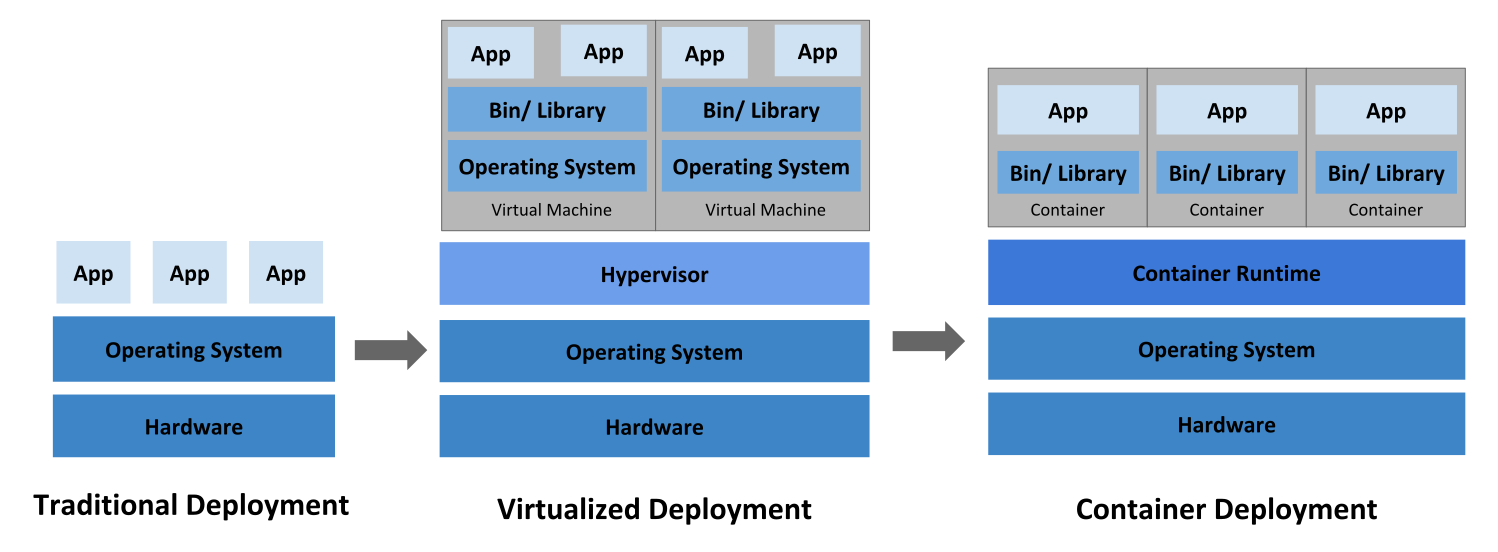
\includegraphics[width=\textwidth]{../imgs/container_evolution.png}
	\captionsource{Evolution of application deployment.}{https://kubernetes.io/docs/concepts/overview/what-is-kubernetes/}
	\label{fig:container-evolution}
\end{figure}

Containers can be thought of as lightweight virtual machines. Unlike the
latter, containers share the same kernel with the host machine but still allow
for a very controlled environment to run applications. There are many
benefits to this : separating the development from deployment, portability,
easy resource allocation, breaking large services into smaller micro-services
or support of continuous integration tools (containers greatly facilitate
integration tests).\\

The CNCF\footnote{\url{https://www.cncf.io/}} (Cloud Native Computing
Foundation) was founded in the intent of leveraging the container technology
for an overall better web. In a general way, we now speak of these
containerized and modular applications as cloud native computing :

\textit{``Cloud native technologies empower organizations to build and run
	scalable applications in modern, dynamic environments such as public,
	private, and hybrid clouds. Containers, service meshes, microservices,
	immutable infrastructure, and declarative APIs exemplify this
	approach.}

\textit{These techniques enable loosely coupled systems that
	are resilient, manageable, and observable.  Combined with robust
	automation, they allow engineers to make high-impact changes frequently
	and predictably with minimal toil.``}\footnote{\url{https://github.com/cncf/toc/blob/master/DEFINITION.md}}

Kubernetes\footnote{\url{https://kubernetes.io/}} is the implementation of this
general idea and was anounced at the same time as the CNCF. It aims at
automating of the process of deploying, maintaining and scaling containerized
applications. It is industry grade and is now the de-facto solution for
container orchestration.


\subsubsection{Kubernetes concepts}
The basic processing unit of Kubernetes is called a \textbf{pod} which is
composed of one or several containers and volumes\footnote{A volume is some
	storage space on the host machine that can be linked to containers, so
	they can read persistent information or store data in the long term}.
In the cloud native context a pod most often hosts a service or micro-service.

\begin{figure}[h]
	\centering
	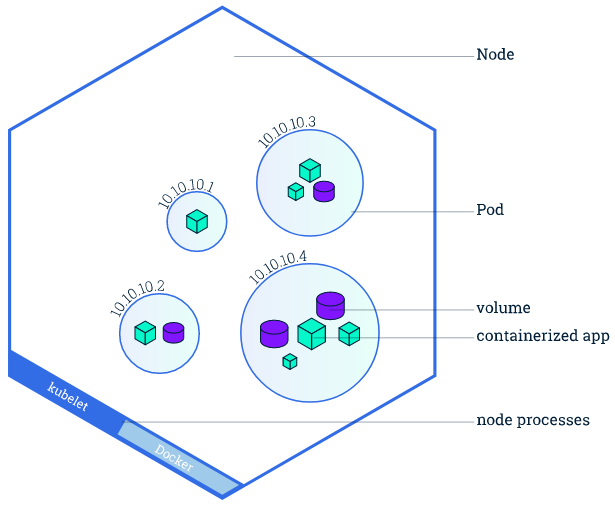
\includegraphics[scale=0.5]{../imgs/node-overview.png}
	\captionsource{Node overview}{https://kubernetes.io/docs/tutorials/kubernetes-basics/explore/explore-intro/}
	\label{fig:node-overview}
\end{figure}

Pods are bundled together in \textbf{nodes} (figure \ref{fig:node-overview})
which are either physical or virtual machines. They represent another barrier
to pass through to access the outside world which can be useful to add layers
of security or facilitate communication between pods. Nodes take the idea of
containerisation further by encapsulating the already encapsulated services.
Each node runs at least one pod and also one \textbf{kubelet} which is a
process responsible for communicating with the rest of Kubernetes (or more
precisely, with the master node which in turns communicates with the api
server). A set of nodes is called a \textbf{cluster}. Each Kubernetes instance
is responsible for running a cluster.

Kubernetes revolves its API server which is its central component (figure
\ref{fig:kube-components}). The majority of operations between components go
through this REST API like user interactions through kubectl or scheduling
operations.

\begin{figure}[h]
	\centering
	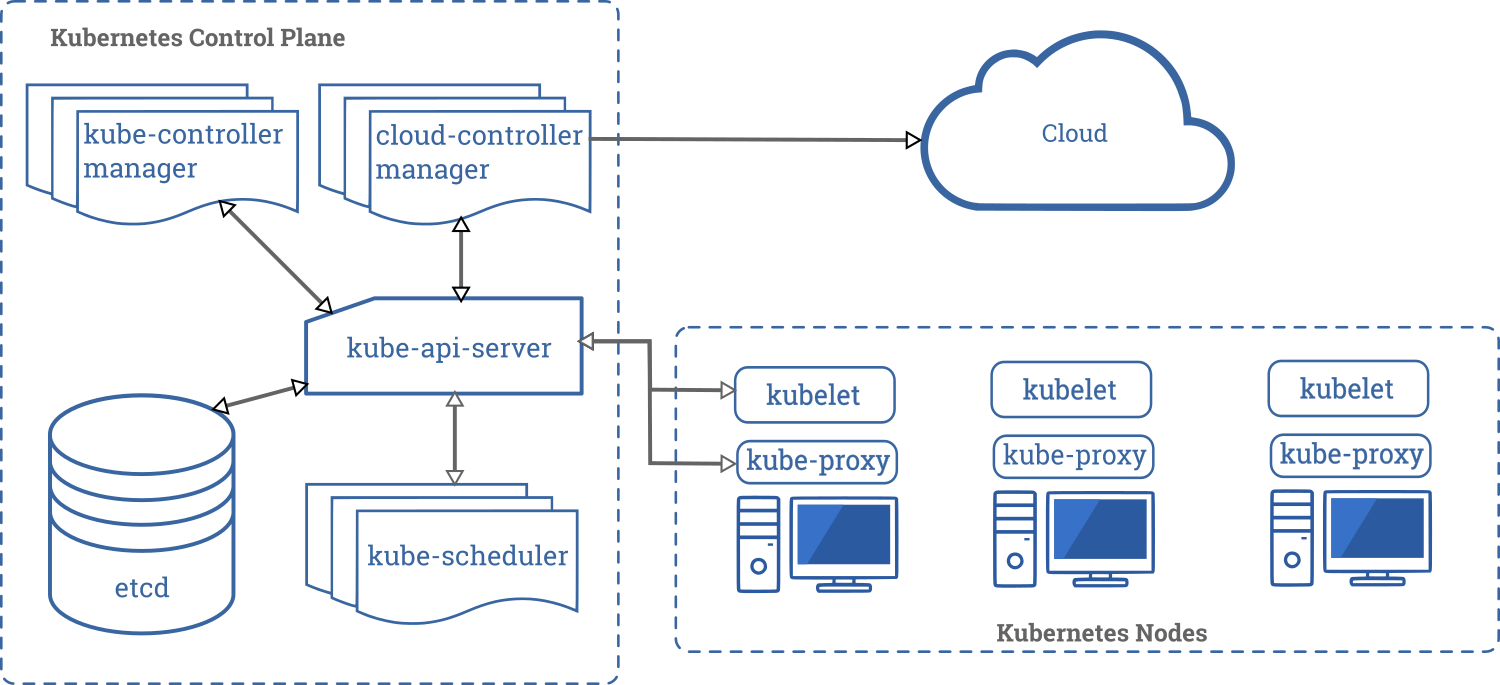
\includegraphics[width=\textwidth]{../imgs/components-of-kubernetes.png}
	\captionsource{Components of Kubernetes}{https://kubernetes.io/docs/concepts/overview/components/}
	\label{fig:kube-components}
\end{figure}

\section{HPC and Kubernetes}
The difference between HPC (High Performance Computing) and Kubernetes lies in
the workloads they are intended to tackle.

A general definition of HPC would be :
\say{\textit{High Performance Computing (HPC) most generally refers to the
		practice of aggregating computing power in a way that delivers
		much higher performance than one could get out of a typical
		desktop computer in order to solve large problems in science,
		engineering, or
		business.}}\footnote{\url{https://wwwen.uni.lu/university/high_performance_computing}}.
HPC can either refer to ``High Performance Computing'' or ``High Performance
Computer'' but it is generally clear which one it refers to, given the
context.

A HPC workload is composed of numerous tasks hungry for computational resources
which are executed in parallel on different machines (that we can refer to as
compute resources or nodes). These tasks may be completely independant like
when different users each submit a single task, or they may also be tightly
coupled together as when a single user submits a job that is composed of
several tasks than can be run in parallel. In that case, the whole system
becomes very sensitive to latency as these tasks have got to communicate
together. This is done through MPIs (Message Passing Interfaces) which
represent a large part of the HPC field.\\

%Kubernetes was designed for cloud native applications.  Services or micro
%services are run in containers and are expected to be available at all times :
%it ensures that containers are restarted when a failure occurs. It also
%provides portability, monitoring and easier administation. It was then
%developed with this objective in mind which hardly complies with the challenges
%of HPC.

%However, there are many issues with the aging HPC field that can be resolved
%with a container driven approach. 
Kubernetes is now the standard for AI and Machine Learning as shown by the many
efforts at making this coupling an efficient
environment\cite{lee2017design}\cite{233001}\cite{10.1145/3154842.3154845},
which brought an increasing interest for container driven HPC aswell and
Kubernetes for HPC in particular. Batch schedulers such as
kube-batch\footnote{\url{https://github.com/kubernetes-sigs/kube-batch}} have
been implemented for kube, and numerous HPC applications like
slurm\footnote{\url{https://slurm.schedmd.com/containers.html}} have been
containerized aswell.

Indeed, containers have many advantages that HPC users can benefit from. Here
are some notable ones:
\begin{itemize}
	\item First off, research has shown that Kuberenetes offer similar
		performance to more standard bare metal HPC\cite{8950981}.
	\item Users will get the same environment everywhere making up for a
		uniform and standardized workplace.
	\item Portability : users could seamlessly hop from one infrastructure
		to another based on their needs and criteria like price,
		performance, and capabilities rather than compatibility.
	\item Encapsulation : HPC applications often rely on complex
		dependencies that can be easily concealed into containers.
\end{itemize}
\begin{figure}[h]
	\centering
	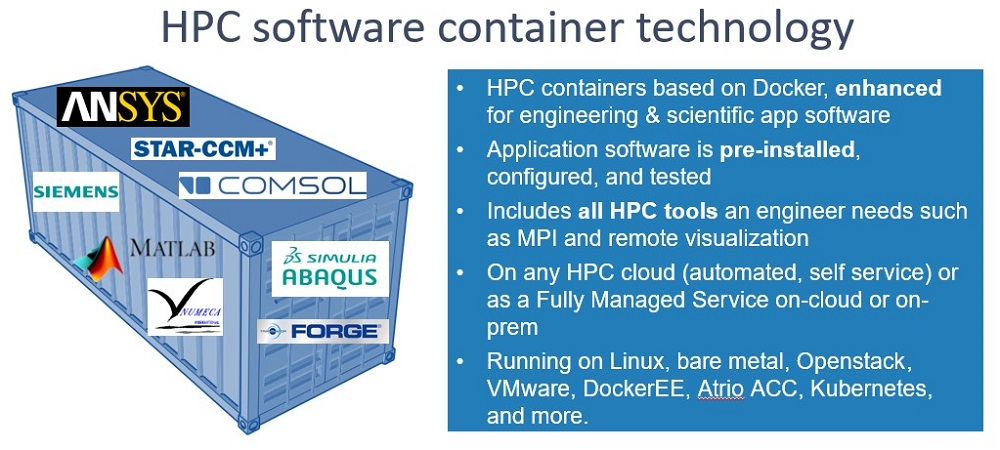
\includegraphics[scale=0.5]{../imgs/hpc-container.jpg}
	\captionsource{The container technology for HPC}{https://www.hpcwire.com/2019/09/19/kubernetes-containers-and-hpc/}
	\label{fig:hpc-container}
\end{figure}

Despite all those advantages, Kubernetes is not ready yet to be used
in proper HPC environment because it lacks vital components like a proper batch
job queuing system, and support for MPI applications. It cannot yet compete
against the very well established HPC ecosystem, however efforts are being made
in this direction. This master thesis is focused on a part of this problem :
Kubernetes simulation for batch schedulers evaluation.

\chapter{The scheduling problem}

\section{Batch scheduling}

\subsection{A general definition}

\subsection{Kubernetes batch schedulers}
\subsubsection{kube-scheduler}
Not exactly a batch scheduler, it is the default scheduler for Kubernetes made
by the CNCF

\subsubsection{kube-batch}
\subsubsection{Poseidon}
\subsubsection{bashScheduler by rothgar}
\subsubsection{random-scheduler by Banzaicloud}
\subsubsection{k8s-custom-scheduler by IBM}
\subsubsection{scheduler by kelseyhightower}


\section{Simulating infrastructures}
\subsection{HPC simulators}
\subsection{Kubernetes simulation}

This raises the question of scheduler development. Developing a scheduler
implies being able to test its performances throughout the development process,
however, testing in real conditions is time consuming and expensive.
Organizations can either have enough resources to cover these costs, or test
their scheduler against a simulation.\\

Kubernetes cluster simulations is an open problem and is the subject of this
master project. Our approach relies on the Batsim\cite{batsim} infrastructure
simulator, which is itself built upon Simgrid\cite{simgrid}. Batsim is
currently mostly used to simulate HPC infrastructures but was designed to be
able to simulate any kind of infrastructure and therefore is theoretically able
to simulate any Kubernetes cluster, moreover, Kubernetes was designed to run
services but is capable of handling High-Performance
Computing\cite{kube-for-hpc}. This project aims at adapting Batsim so it can
evaluate Kuberenetes schedulers.

\section{The Batsim infrastructure simulator}
\subsection{Batsim concepts}

\subsection{Limitations}


\chapter{Problematic}

\section{Objectives}

The goal of this project is to design and implement Batkube, which will be an
interface between Batsim and Kubernetes schedulers. With this interface, we
want to compare Batsim results gainst data from a real Kubernetes cluster,
given HPC workloads.

\section{Translation}

\section{Synchronization}

\chapter{Implementation}

\section{Batkube architecture}
TODO

\section{API implementation}
\section{Time hijack}
TODO

\subsection{batsky-go}
\SetKwInput{KwInput}{Input}
\SetKwInput{KwOutput}{Output}


\begin{algorithm}[H]
\DontPrintSemicolon
\KwInput{req: request channel, res: result channel map}
\While{Batkube is not ready} {
	wait\;
}
requests = []request\;
\While{req is not empty} {
	m = $<$- req \tcc{Non blocking receive}
	requests = append(requests, m)\;
}
sendToBatkube(requests) \tcc{Only requests with duration > 0 are actually sent. Batkube will always anwser.}
now = responseFromBatkube()\;
\For{m in range requests} {
	res[m.id] $<$-now \tcc{The caller continues execution upon reception}
}

	
\caption{Requester loop}
\label{alg:reqLoop}
\end{algorithm}


\begin{algorithm}[H]
\DontPrintSemicolon
\KwResult{Current simulation time}
\KwInput{d: timer duration, req: request channel, res: response channel map}
\KwOutput{now : simulation time}

\If{requester loop is not running}{
	go runRequesterLoop() \tcc{There can on ly be one loop runing at a time}
}
id = newUUID()\;
m = newRequestMessage(d, id) \tcc{Requests are identified using uuids}
resChannel = newChannel()\;
res[id] = resChannel \tcc{A channel is associated with each request}
req $<$- m \tcc{The code blocks here until request is handled}
now = $<$-resChannel \tcc{The code blocks here until response is sent by the requester loop}
return now\;
\caption{Time request (time.now())}
\label{alg:now}
\end{algorithm}



\chapter{Evaluation}

\chapter{Conclusion}


\printbibliography
\end{document}
